\section{\texorpdfstring{Symmetric ciphers, DES, AES}{Symmetric ciphers, DES, AES}}
\vspace{5mm}
\large

\subsection{Symmetric Ciphers}
There are 2 kinds of symmetric ciphers: block and stream.

\begin{definition}
	Block ciphers work on fixed-size blocks of $b$ bits.
	\[ E:\{0,1\}^b \times \{0,1\}^k \to \{0,1\}^b \]
	Therefore, encryption is a bijection (permutation on set of block values).
\end{definition}

\begin{definition}
	Assume an attacker is given an oracle which contains either $E_k$ with random key $k$ or a random permutation.
	Block cipher is secure iff an attacker cannot distinguish what is inside the oracle.

	More precisely: does not exists a distinguisher with $Pr[$success$] \geq 2/3$ and run time $< 2^{security\ level}$.
\end{definition}

\begin{definition}
	Substitution-Permutation Network (SPN) is an iterated cipher where each round consists of:\\
	1) S-boxes of bijective substitution (confusion)\\
	2) P-box (permutation) on positions (diffusion). Typically permutation is an involution: $\pi \circ \pi = id$.\\
	3) Mixing round key $k_i$ by $\oplus$.

	\includegraphics[scale=0.3]{spn_0.eps}

	1 Round:

	\includegraphics[scale=0.4]{spn_1.eps}

	Round is invertible. Inverse of SPN is again an SPN.

\end{definition}

\subsection{DES}
DES contains Feistel network with 16 round, 64-bit blocks, 56-bit keys.

\paragraph{Feistel network (1 round):}

	\includegraphics[scale=0.4]{des_0.eps}

Where $f$ is non-invertible function called Feistel function. $K_i$ is a new key derived from master, one per round.

\paragraph{Feistel function:}

	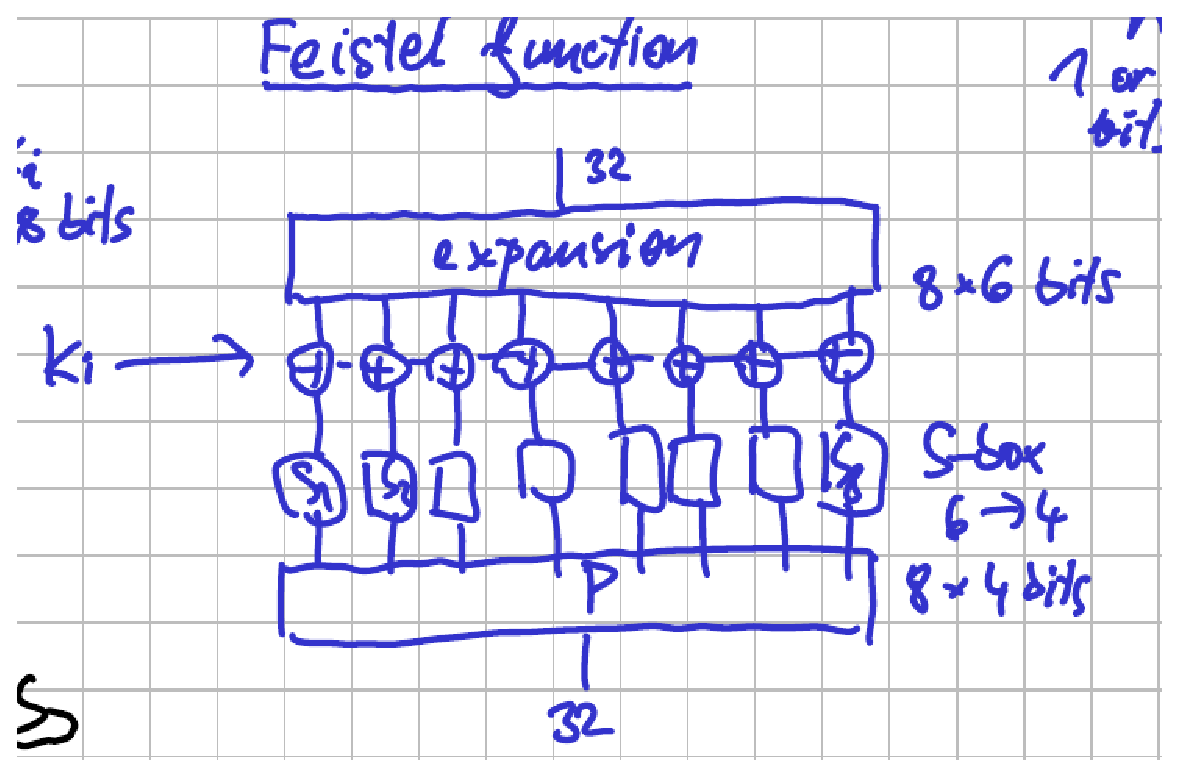
\includegraphics[scale=0.4]{des_1.eps}

Where expansion splits input into groups of 4 and takes 2 bits from neighbours.

	\includegraphics[scale=0.4]{des_2.eps}

\paragraph{Key schedule} Produces new keys per round:

	\includegraphics[scale=0.4]{des_3.eps}

Bit mapping discards parity bit and permutes the rest. As a result key is 56b, instead of 64b as formal definition.
Key schedule produces a new key, also sends output to the new round (of key schedule).

2nd mapping box is the same for all round in Key schedule, the only difference is in the \# of rotations in $<<$ (1 or 2 bits rotation).

As a result every $K_i$ is a subset of master key, permuted in some way.

Critique of DES:
\begin{enumerate}
	\item Weak keys. If $K = 0^{56} \Rightarrow \forall i: K_i = 0^{48}$, so $\oplus$ after Feistel function has no effect and all rounds are identical. Same for all 1s.
	\item $E_{\overline{k}}(\overline{X}) = \overline{E(x)}$. Random symmetric cipher does not have this property.
	\item Short key. Brute force attack is feasible (26 hours in 2012).
		Solution: use 2-DES or 3-DES.

		2-DES contains 2 round of DES. Does not improves security level significantly, only to $2^{57}$.
		With that many steps known plain and cipher text we can break the key.

		3-DES: $E_{k_1}(D_{k_2}(E_{k_3}(x)))$. Which is slow, security level is $\leq 113$, 168 bits of key.

	\item Too short blocks: in $2^{32}$ block collision will occur.
		Solution: change the key after $\approx$ mln of blocks.
	\item Too much secrets (NSA changed s-boxes last minute)
	\item Attacks on structure ($2^{47}$ chosen plain text)
\end{enumerate}
To conclude, DES is dead!.
\subsection{AES}

\begin{definition}
	AES - advanced encoding standard, known as Rinjdael. Has 128 bit blocks, multiple key lengths in standard:\\
	1) 128b (10 rounds)\\
	2) 192b (12 rounds)\\
	3) 256b (14 rounds)

	Internal structure: SPN with linear step.

	Internal state: matrix $M \in GF(2^8)^{4 \times 4}$.
\end{definition}

AES round:
\begin{enumerate}
	\item (S) Byte sub (16 identical s-boxes). Does inversion in GF + affine transformation.
	\item (P) Shift rows. //TODO picture
	\item (L) Mix columns: liner transformation on every column
	\item $\oplus$ XOR with $K_i$.
\end{enumerate}
 Decryption does inverse:
\begin{enumerate}
	\item $\oplus$ XOR with $K_i$.
	\item (L) Inverse Mix columns (additional linear step): liner transformation on every column
	\item (P) Inverse Shift rows.
	\item (S) Inverse Byte sub (s-box should be invertible).
\end{enumerate}

\begin{observation}
	(S) and (P) commute, order can be changed.
	We can also swap XOR and Inverse mix columns with a key modification.

	Consequently, D and E differ only in cleanup.
\end{observation}

\begin{note}
	SW implementation of AES could be speeded up by precomputing Byte sub as lookup table.
	Also precompute
	\begin{gather*}
		m_1(x) = mix(s(x), 0, 0, 0) \\
		m_2(x) = mix(0, s(x), 0, 0) \\
		m_3(x) = mix(0, 0, s(x), 0) \\
		m_4(x) = mix(0, 0, 0, s(x))
	\end{gather*}
	Then mix is
	\[ mix (s(x_1), s(x_2), s(x_3), s(x_4)) = m_1(x_1) \oplus m_2(x_2) \oplus m_3(x_3) \oplus m_4(x_4) \]

	Requires only 1kb of precomputed values. However can be attacked because of cache properties.
\end{note}

Critique of AES:
\begin{enumerate}
	\item Simple algebraic structure (LA + finite fields) $\Rightarrow$ could lead to system of Linear equations that could break the key.
	\item Small margin in \# of rounds. (Many attacks start with less rounds e.g. 6 and succeed, than increase number of rounds)
	\item Byte alignment. All operation are on whole bytes $\Rightarrow$ diffusion and confusion are much faster across bytes than inside.
	\item 128-bit key can be attacked by quantum computers using Grover alg. Which requires $\sqrt{n}$ steps comparing to $n$ steps of brute force.
	\item 128-bit blocks $\Rightarrow$ collisions in $\approx 2^{64}$ blocks.
		Solution: change key after $2^{32}$ blocks.
\end{enumerate}

\subsection{Usage and Modes of Block ciphers}

Because of the block cipher properties we need:\\
1) Padding that can be reversed.\\
2) Split message into blocks

\begin{definition}
	ECB - electronic code book. Encrypts all blocks independently in parallel.

	\includegraphics[scale=0.4]{ecb.eps}

	Avoid at all costs:
\begin{enumerate}
	\item No IV.
	\item Encryption is the same for identical inputs.
	\item Reveals $x_i = x_j \Rightarrow y_i = y_j$ blocks.
	\item Attacker can change 1 bit in $y_i \Rightarrow$ destroys $x_i$.
	\item Swap $y_i = y_j \Rightarrow$ swaps $x_i = x_j$.
\end{enumerate}
\end{definition}

\begin{definition}
	CBC - cipher block chaining.

	\includegraphics[scale=0.4]{cbc.eps}

	Properties:
\begin{enumerate}
	\item Requires random IV.
	\item Bit flip in $y_i \Rightarrow$ destroys $x_i$ and flip in $x_{i + 1}$.
	\item Block swap gives predictable result:
		\[ y_i \iff y_j \Rightarrow x_{i + 1} = y_i \oplus y_j \land x_i = x_j \oplus y_{i-1} \oplus y_{j - 1} \]
	\item Proof of security for chosen plain text.
		CBC is secure even using not ideal cipher for short messages $\leq (\sqrt{block\ space\ size} \cdot numb\ blocks)$.
\end{enumerate}

\end{definition}
\begin{definition}
	CTR - counter.

	\includegraphics[scale=0.4]{ctr.eps}

	Properties:
\begin{enumerate}
	\item Behaves as stream cipher $\Rightarrow$ no need of padding.
	\item Cannot use same IV twice.
	\item Bit flit in $y_i \Rightarrow$ bit flip in $x_i$.
		Should be handled by protocol.
	\item Random access + parallelizable $\Rightarrow$ suitable for disk encryption.
\end{enumerate}
\end{definition}

\begin{definition}
	OFB - output feedback.

	\includegraphics[scale=0.4]{ofb.eps}

	A short cycle of permutations could occur $\Rightarrow$ reduces \# of IVs as we cycle.
\end{definition}

\begin{definition}
	Cipher text stealing - trick to avoid using predictable padding pattern for block ciphers. We use plain text data to complete last block.

	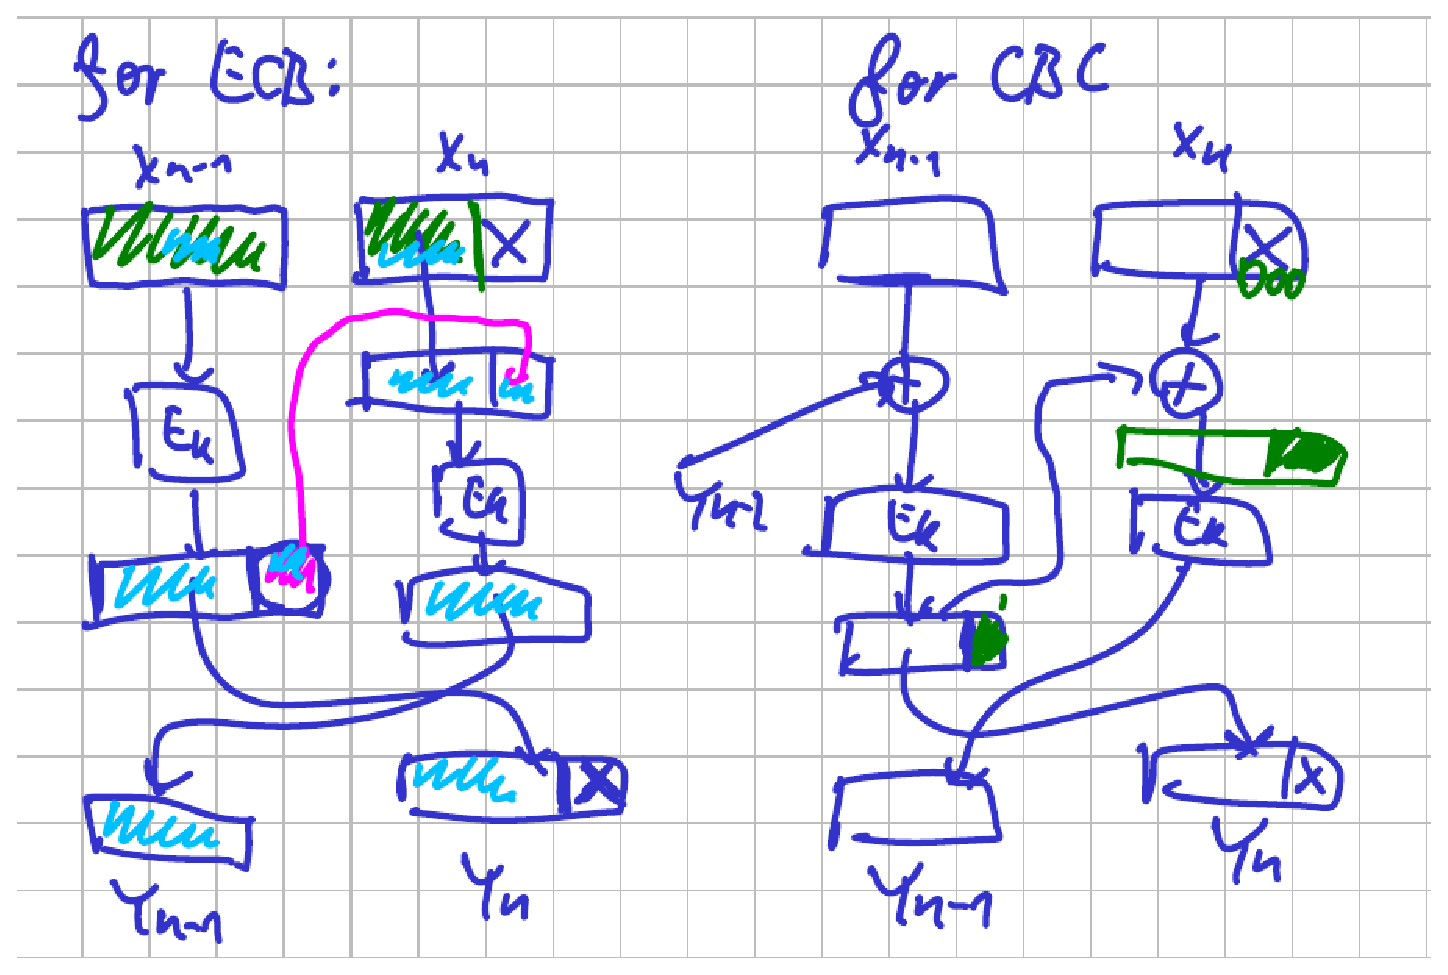
\includegraphics[scale=0.4]{steal.eps}
\end{definition}

All block ciphers leak some information, which is significant.
\begin{enumerate}
	\item ECB: $x_i = x_j \Rightarrow y_i = y_j$.
	\item CBC: $y_i = y_j$ is likely to happen after $2^{b/2}$ blocks. Also
		\[ E_k(x_i \oplus y_{i - 1}) = E_k(x_j \oplus y_{j - 1}) \Rightarrow  x_i \oplus y_{i - 1} = x_j \oplus y_{j - 1} \Rightarrow x_i \oplus x_j = y_{j - 1} \oplus y_{i - 1} \]
		$b$ bits are known to attacker per $\approx 2^{b/2}$ blocks.
		Solution: do not use a single key for encryption of $2^{b/2}$ blocks.
	\item CTR: Assume $C_1, ..., C_m: C_i = E_f(IV + i - 1)$. All $C_i$ are different, so
		\[ y_i \oplus y_j = (x_i \oplus C_i) \oplus (x_j \oplus C_j) = (x_i \oplus x_j) \oplus (C_i \oplus C_j) \land C_i \oplus C_j \neq 0 y_i \oplus y_j \neq x_i \oplus x_j\]
		Rules out 1 of $2^b$ possibilities for every pair. And the difference in entropy per pair is:
		\[ b - log (2^b - 1) = \log\left(\frac{2^b}{2^b - 1}\right) = \log\left(1 + \frac{1}{2^b - 1}\right) \approx c 2^{-b} \]
		So \# of bits leaked $\leq \binom{m}{2} \cdot c \cdot 2^{-b}$, const for $m \approx 2^{b/2}$.
\end{enumerate}

\subsection{Padding oracle attack}

Assume, we use an padding pattern with $p$ block filled with value $p$ in every byte.
Attacker has access to an oracle (e.g. server) that for given cipher text answers whether padding was correct, or data is corrupted.
For example by a return code (500), alternatively attacker can measure how long it took to process the data (time attack).

Because of the CBC mode structure, changing $y_{n-1}$ block (which is XORed with decrypted $y_n$) changes last block of plain text.
Assume $p\neq 1\Rightarrow$ last byte is not $01$. An attacker can give server all possible values of the last byte to get $01$ in the decrypted plain text.
If we guessed such value, we get last byte of decrypted $y_m$ (intermediate state). The last step is to XOR initial $y_{n-1}$ with intermediate state we have. Doing so we obtain last byte of plain text, which is not only equal to padding, but also reveals how many block of padding plain text had.

Attack will continue by changing cipher text to get padding equal to $(p+1)$ till we reach maximum possible padding. Then attacker just removes the last block of cipher text and repeats first phase of attack.

Time complexity of the attack is $b \cdot 2^8$ where $b$ is \# of bytes per block.

	\includegraphics[scale=0.4]{oracle.eps}

\subsection{Stream ciphers}

	\includegraphics[scale=0.3]{stream.eps}

\begin{example}
	LFSR - Linear Feedback Shift Register.

	\includegraphics[scale=0.3]{lfsr.eps}

	Implementation is trivial in HW (bit shifts + XOR). However, LFSR can be cracked by Known plain text attack.
\end{example}

Attempts to save LFSR:
\begin{itemize}
	\item non-linear feedback (\&)
	\item non-linear output (e.g. using hash function).
	\item combine multiple registers and hash together.
	\item control clock of LFSR using second register.

	\includegraphics[scale=0.3]{lfsr_0.eps}
\end{itemize}

\begin{example}
	ChaCha20 is a stream cipher developed by Bernstein. Consists of 20 rounds.
	Has 256b key, 64b nonce, 64b block counter. A non-bijective function $f$ converts these inputs into 1 block of keystream.

	\includegraphics[scale=0.3]{cha.eps}

	Salsa20 is the upgraded version of ChaCha20.
\end{example}
